\documentclass[sigconf]{acmart}

\usepackage{graphicx}
\usepackage{hyperref}
\usepackage{todonotes}

\usepackage{endfloat}
\renewcommand{\efloatseparator}{\mbox{}} % no new page between figures

\usepackage{booktabs} % For formal tables

\settopmatter{printacmref=false} % Removes citation information below abstract
\renewcommand\footnotetextcopyrightpermission[1]{} % removes footnote with conference information in first column
\pagestyle{plain} % removes running headers

\newcommand{\TODO}[1]{\todo[inline]{#1}}

\begin{document}
\title{Using Big Data to Minimize Fraud, Waste, and Abuse (FWA) in United States Healthcare}


\author{Paul Marks}
\affiliation{%
  \institution{Indiana University}
  \streetaddress{Online Student}
  \city{Shepherdsville} 
  \state{Kentucky} 
  \postcode{40165}
}
\email{pcmarks@iu.edu}


\begin{abstract}
The cost of healthcare includes the loss of billions of dollars due to Fraud, 
Waste, and Abuse (FWA).  Many of the schemes to commit FWA are very intricate and 
require the analysis of many data sources simultaneously.  The question answered 
here is ``How can we use big data analysis to help minimize these costs and thus 
optimize the money spent on healthcare?''
\end{abstract}

\keywords{i523, hid327, fraud, waste, abuse, healthcare, health insurance}


\maketitle

\section{Introduction}

FWA is an issue that affects everyone in the U.S. since healthcare services are 
leveraged by everyone at some point and the costs for those services include the 
money lost to FWA.  The three components of FWA are varying degrees of 
culpability.  The Centers for Medicare and Medicaid Services (CMS) in part defines 
fraud as ``knowingly and willfully executing, or attempting to execute, a scheme or 
artifice to defraud any health care benefit program'', Waste as ``overusing services, 
or other practices that, directly or indirectly, result in unnecessary costs'', and 
Abuse as ``involves payment for items or services when there is not legal entitlement 
to that payment and the provider has not knowingly and/or intentionally 
misrepresented facts''.\cite{MLNFWA}  While the percentage of cost attributable to 
FWA can vary from insurer to insurer, Medicare estimates that 11 percent of its 
payments for Original Medicare are improper primarily due to FWA.\cite{FY2016HHSFR}  
In combination these cost the United States healthcare system 80 billion 
dollars\cite{HFMA} annually.  

Advances in big data technology can help reduce these losses.  Big data offers the 
ability to look at data in real time to determine if a claim is legitimate or not.  
Historically, due to the amount of data involved, this type of analysis would have to 
happen after the claims have been paid with specific models targeting specific 
schemes to identify FWA.  Big data can help lower the cost of health-care in the 
United States by identifying FWA claims and stopping payments before they occur. 


\section{Healthcare Fraud, Waste, and Abuse Environment}

It is easy to understand the problem FWA poses.  Healthcare funds are of limited 
quantity.  Insurance helps to spread the cost among groups of people, but does not 
provide limitless funds.  As costs increase, so do premiums or direct payments for 
healthcare.  In order for as many people as possible to be able to have access to 
healthcare costs have to be managed.  There are many ideas for helping to provide 
affordable healthcare, but there is much discussion and disagreement on exactly how 
to do that.  Reducing costs by eliminating as much FWA as possible is one solution 
that everyone, except for those participating in and profiting from FWA schemes, 
can agree on.

Data to fight FWA is not just the information gathered by a doctor or other provider 
while working with a patient.  In order to fully utilize advances in technology, 
multiple sources of information must be brought together.  Sources include claims 
(current and historic), clinical, provider, geospatial, and other sources of 
information.  This allows for data analytics to take a deeper look into not only a 
single participant, but others who may be related to that participant.  Providers who 
are involved in improper billing tend to be associated with other providers who have a 
higher frequency of being involved with improper billing as well.  For big data analysis 
this involves looking at corporate ownership, who providers use as a billing agent, and 
who they tend to refer patients to for other service in order to uncover a larger 
pattern of FWA collusion.\cite{RevCycle}

The problem for big data to solve is the size of all this data and how to process it 
fast enough.  Using CMS as an example, being a government entity much of their data is 
available publicly, it is easy to get an idea of the amount of data.  Medicare processed 
1.2 billion claims in 2014, covering 53.8 million beneficiaries, with 6,142  
hospitals, and 1,173,802 non-institutional providers\cite{2015CMSStatistics}.  In addition
payments must be made within a specific timeframe depending on the insurer and their 
agreement with providers.  This time includes all the normal steps to verify and process 
a claim so the time available to examine the data for FWA is very limited.

It must be noted that when working with this type of data, Protected Health Information
(PHI) and Personally Identifiable Information (PII), that there are many regulations about
the ability to access and secure it which must be followed.  While this makes it more
difficult to get access to the data it can be overcome by working cooperatively with the 
various data owners.  
  

\subsection{Big Data Techniques for FWA}

So how can big data be used to approach this issue?  Leveraging big data tools such as 
Hadoop, analysts could divide the different sources of information into data lakes, 
looking at each source separately, and then combining the results.  Table 
\ref{fig:TypesofFraud} on page \pageref{fig:TypesofFraud} shows sources of information 
and what level of FWA they are generally related to.  The highest level combines sets 
of data from all data views.  It looks for patterns across criminal networks which may 
involve many providers and beneficiaries.  By looking at things more globally across 
potentially billions of records, big data provides the ability to perform complex 
network analysis which can uncover intricate conspiracies perpetrated by coordinated 
efforts of many providers and facilities.\cite{THORNTON20131252} 

While there are simple cases of fraud which follow 
a typical known pattern, this is only a portion of the problem.  Fraud schemes 
change and can involve many different entities which may not seem to be related on the 
surface.  The more data which can be combined and analyzed, the more fraud that can be 
found.  The need for this type of analysis is because much of the FWA committed in 
healthcare is done so by providers working in conjunction with each other and providers 
working in conjunction with their patients.\cite{LexisNexis}  Big data analytics can 
find hidden relationships and patterns in information which show FWA clusters.  These 
can include, but are not limited to:  
\begin{itemize}
  \item Relationships between patients and the people who are committing fraud,
  \item Connections among those committing fraud, employees, businesses, and even their 
  relatives,
  \item Suspect interactions between providers, and
  \item Overall inappropriate relationships among various active fraud participants, 
  partners, and patients.\cite{LexisNexis}
\end{itemize}
In order to keep up with organized fraud activities, there must be a dedicated practice 
of data analytics which is ever evolving. 

Traditionally programs have been written to look for specific sets of circumstances.  
Leveraging existing knowledge about the data and using it to look for specific patterns 
is known as supervised in big data terms.  Supervised fraud detection is represented 
in several methods including ``Bayesian Networks, Neural Networks (NNs), Decision Trees, 
and Fuzzy Logic.''\cite{Ghuse}  Neural Networks and Decision Trees have a higher 
tolerance for handling large amounts of noisy data and are therefore more popular than 
the other methods.  There are also unsupervised methods in which data is fed into the 
system without preexisting notions of what to look for\cite{Ghuse}.  Unsupervised 
methods sort through data and find relationships and groupings of related information, 
find clusters of what could be considered normal, and determine where the outliers are.

Because unsupervised methods only identify outliers, applying unsupervised methods to 
healthcare data requires that outliers then have to be verified as FWA or 
acceptable patterns.  According to Anthem's SVP of Healthcare Analytics Patrick 
McIntyre, they take this into account.  Anthem is able to run algorithms against their 
claims as they are being processed.  This allows machine learning to discover claims 
which may be fraudulent or wasteful in nature on a daily basis.  Once identified 
``questionable claims are immediately identified, flagged and sent to the clinical 
coding experts for review.''\cite{Datameer}  This greatly increases the ability to 
fight FWA by having the machine pinpoint where to look in all the data available to 
the reviewer.  Suddenly the task of finding fraud is not as daunting.  By leveraging 
both of these techniques FWA can be discovered at an accelerated pace.  The number of 
models the system knows will grow over time as more data is fed into it and more 
patterns are discovered and verified.


\subsection{Current Solutions}

Many companies currently offer solutions for detecting FWA in healthcare payment systems. 
They include the ability to identify FWA claims during the payment cycle so that payment 
is not made to suspect claims.  Truven Health\cite{TruvenHealth}, Healthcare Fraud Shield\cite{FraudShield}, 
and SAS\cite{SASHealth}, just to name a few, all have systems they offer based on big data.  The 
specifics of the systems they offer are proprietary in nature so many of the descriptions are 
generic.  Truven Health claims their solution mixes technology and healthcare intelligence.  They 
have a model which groups services together for form a picture of the full view of the illness 
including inpatient, outpatient, and pharmaceuticals. This data in analyzed by knowledge rules based 
on clinical classifications and medical literature.  This helps to identify wasteful or unnecessary 
service patterns in clinical and billing abuse which are hard to detect.  Using this approach 
an analyst can look at the costs associated with the patient during their illness, the services 
provided, and combine this with others to form a profile of the provider's practice.\cite{TruvenHealth}

SAS materials include the ability to find hundreds of millions of dollars in savings before 
claims are paid by taking an enterprise approach to FWA.\cite{SASHealth}  Their solution 
incorporates the rules and models into the claims process so companies can process the rules 
against all of their claims instead of sample sets.  This helps to uncover more schemes and 
``spot linked entities and crime rings, which can help stem larger losses.''\cite{SASFraud}.  
Recently the Centers for Medicare and Medicaid Services awarded Northrop Grumman Corp. a contract 
worth \$91 million to develop a second generation advanced analytics system to fight FWA in 
Medicare and Medicaid by identifying high-risk claims.\cite{ModernHealthcare}

\subsection{Future uses of Big Data Analytics}

Currently there is still a certain amount of honor built into healthcare.  The inherent 
structure of the healthcare reimbursement system allows for both billing errors and 
fraudulent actors to go undetected, taking money away from the system set up to pay 
legitimate claims.\cite{RevCycle}  If a claim is submitted by a valid entity, using the 
correct process, and everything is in order then it is most likely paid.  For many claims this 
is done without any specific proof of the services being provided.  With more and more 
healthcare information being digitized this may not be the case in the future.  X-rays, lab 
tests, clinical notes, etc. are all being stored digitally.  Computers are now able to interpret 
images and unstructured text very accurately.  By linking this data to claims data the clinical 
information could be required as part of claims payment.  An x-ray of broken bone, notes which 
support a diagnosis, Magnetic Resonance Imaging files, could all be interpreted automatically.  
Not only would the data be used to compare to the claims information, but to other images/notes 
on file to ensure that the same files were not being submitted with multiple claims.  The system 
could know what one individual medical history looks like compared to another similar to how 
facial recognition is able to match like images.  Requiring and being able to validate more 
information before services are paid for would help the reduce the ability of perpetrators of FWA 
to be able to get reimbursed for services they should not.  This level of verification would not 
be possible without the ability to process massive amounts of data quickly.  


Historically the payers of most healthcare claims, insurers, have not had the 
ability to examine actual evidence that a service has taken place on a broad scale.  (It is done 
manually on a specific case or audit basis.)  Through the use of advances in big data and combining 
current and new data stores such as electronic health records into the payment process, a difference 
can be made in the amount of money lost to FWA in healthcare.  Data from providers must be run 
against entity resolution solutions.  Complex claims analysis, including rules-based clinical 
reviews, must be part of the normal pre-payment workflow leveraging predictive analytics to 
stop payments on billions of dollars worth of FWA claims before they are made.  The FWA problem 
goes beyond healthcare.  It is ``a national economic imperative that must be addressed 
immediately.''\cite{LexisNexis}  The technology exists today that can help protect the
integrity of the healthcare system and the quality of care for Americans. \cite{LexisNexis}


\section{Conclusions}

While there may be disagreement on many aspects of healthcare in America, everyone should agree 
that eliminating Fraud, Waste, and Abuse within the system is the right thing to do.  FWA costs 
billions of dollars annually.  Just a 1 percent reduction in the estimated 80 billion dollars 
annually would result in 800 million dollars in savings.  With this amount of money at stake 
significant investments should continue to be made in leveraging advanced big data technologies 
into solving this problem.  Due to the continued rise in the amount of data collected traditional 
programming cannot keep up with the pace.  Advanced techniques must be leveraged which can learn 
in an unsupervised manner.  The future of the best methods for fighting FWA in healthcare will be 
a combination of this analysis and teams specializing in the rules and regulations of healthcare
in the United States.  The unsupervised methods will work through massive amounts of structured and 
unstructured data breaking it down into cases and schemes which are most likely FWA.  These will be 
reviewed, confirmed or denied as accurate, and fed back into overall FWA platform.  As this cycle 
continues over and over the ability to fight FWA in United States Healthcare will get better.  
While Big Data may never eliminate FWA in Healthcare it can help to minimize it and save the
country billions of dollars a year.

\begin{acks}

  The author would like to thank Dr. Gregor von Laszewski for his
  support and suggestions to write this paper.  It has helped to expand my knowledge in how modern 
  data analytics can help to save FWA which has plagued the healthcare system.

\end{acks}

\bibliographystyle{ACM-Reference-Format}
\bibliography{report} 

\begin{table}[htb]
    \caption{Types of Fraud and their related Sources\cite{THORNTON20131252}}
    \label{fig:TypesofFraud}
    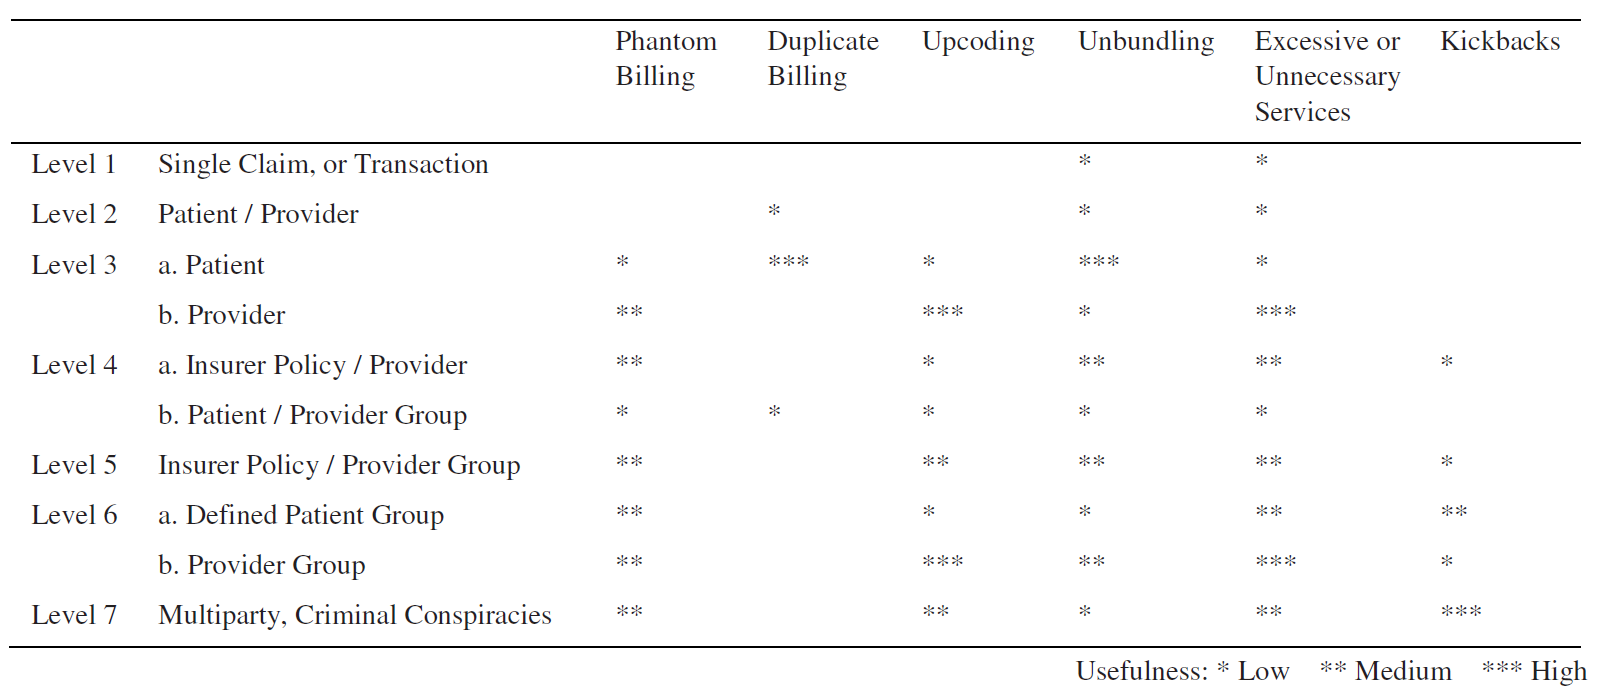
\includegraphics[scale=0.60]{images/TypesofFraud.png}
\end{table}


\end{document}
